\documentclass[main.tex]{subfiles}
\begin{document}

\section{Addition of path finding algorithm}

\subsection{Practical motivation}
While the main aim of the application developed by this project was to actively track user movement within a building, we realized that making use of path finding will greatly benefit the project as well. This resulted from information obtained from other sources, where certain positions in buildings were utilized in order to reset the error caused by the sensors. On top of that, this addition resulted in an easier to understand interface as well as aiding the user in the search for their destination. In order to add a path finding algorithm to our project, we decided to investigate the different available options and evaluate their performance in order to identify the optimal algorithm.

\subsection{Path finding algorithms considered}
The previous sections detailed how we extracted a graph structure from the image data provided for each floor. This graph structure can be thought of as a mesh, representing walkable areas of the floor via vertices and edges. There are several algorithms that are capable of performing path finding on this type of data-structure and we selected the most popular ones for our testing. 

\subsubsection{Dijkstra}
This is a shortest path graph path finding algorithm. While there are many iterations, the two major versions differ greatly. Initially, this algorithm searched for the path only between the two specified nodes (start and end node), however the later versions, being the more prevalent ones nowadays, perform this kind of calculation on all nodes in the graph. This means that if we specify a node within the graph as our finish node, the algorithm will calculate the shortest path from all of the other nodes in the graph to this node. While this seems inefficient, the reason for this is the minimal performance hit incurred by performing this operation, as well as the possibility of these results being reused at a later run of the algorithm. These kinds of implementation therefore make heavy use of caching.
The base runtime of Dijkstra's algorithm is $O(V^2)$, where V is equal to the number of vertices in the graph. This can however be further optimised by using the altered implementation of the algorithm by Fredman \& Tarjan\cite{algoImprovedDijkstra}, where the implementation is based on a min-priority queue that makes use of a Fibonacci heap. This kind of implementation runs in $O( E + V + log(V) )$ , where E stands for the number of edges in the graph and V stands for the number of nodes. Thanks to this change in implementation, Dijkstra is one of the fastest shortest path algorithms that can be used for arbitrary directed graphs with a single restriction that dictates that edge weights have to be non-negative.


\subsubsection{A*}
A* is an informed graph search algorithm that makes use of heuristics.  An informed algorithm functions on the premise of solving a problem by searching for the solution amongst all of the solutions available for a given graph. While this might seem inefficient as there can be millions of ways to traverse a graph, A* employs two measures to greatly reduce the subset of solutions. It does this by utilizing two measures for each node:
\begin{itemize}
\item g(n) - This function represents the cost of the path required to reach a specific node n. A cost in this case can be anything ranging from distance to petrol required to travel. Using this function ensures that any specific solution is aware of the requirements to get into the state it is in.
\item h(n) - Represents the estimated cost of travelling from a specific node n to the target finish node. We can use multiple estimation techniques depending on the knowledge of environment, such as Manhattan distance or Euclidean distance.
\end{itemize}

The strength of A* comes from combining the two measures explained above into a single measure, allowing the algorithm to estimate the best partial move when traversing a graph. This makes A* a very flexible and strong candidate for path finding on graphs. Therefore, it is also highly favoured in games.

\subsubsection{Recast}
The last algorithm considered was the Recast\cite{libRecast} algorithm, now commonly used in games. It originates from a game navigation construction toolkit. The recast approach makes use of heavy pre-processing of the input meshes. The only restriction for the input mesh is for it to consist of triangles, this is then pre-processed into voxel mold, which then in turn allows the algorithm to estimate walkable spaces and perform a conversion to convex polygons. Once the conversion is complete, Recast is then able to make use of the polygons to reason about walkable space, taking into account measures of an agent (such as height or width).
\newline

Recast offers a great deal of flexibility and has an excellent turnaround time. The fact that it allows for real-time modification of the mesh and is able to respond to changes in it further allows for possible extensions of the project such as obstacle detection (for example moved furniture) or others. While this does require additional levels of pre-processing, the potential performance gain is significant enough to benchmark this algorithm.

\subsection{Existing libraries}
Due to the fact we decided to develop in C\# and make use of Xamarin studio, we were able to locate PCL compliant libraries able to be deployed on our mobile devices. These libraries make use of our previously pre-processed graph data structure that can be interpreted as a mesh. This allowed us to easily adapt our extracted data to the needs of each library we investigated. Each library we tested offered a different implementation of one (or multiple) of the algorithms mentioned above. As discussed before, some implementations make use of caching in order to speed up their subsequent operation, while others focus on refining the data structures that are responsible storing the graph representation. This allowed us to observe the impact of the two solutions on the mobile device.

\subsubsection{SharpNav}
This library\cite{libSharpnav} is a PCL compliant non-native port of Recast. The version we used was labelled "SharpNav.Mono" which was able to be run on our Android devices. Our tests conducted using this library have shown promise, however due to the early stage of development of this library, its PCL variant offers very little support when it comes to loading pre-processed data. This would mean we have to do all three stages of pre-processing on the device, which was not acceptable due to the long time required to do so. This also required all three of the data structures (mesh, voxel mold and convex polygon representation) to be stored in the device memory, resulting in the host application encountering memory related issues. We were therefore forced to move away from using this library, as it wasn't a good match for a limited space a mobile app has allocated.

\subsubsection{Urho3D}
The second option we considered was the Urho3D game engine, which is partially developed by programmers at Xamarin. This engine\cite{libUrho} is capable of creating, saving, and performing operations on a mesh pre-processed by Recast. In order to utilize these elements of the engine, we were required to create test applications containing other base elements first. Therefore, we quickly realized that, in order to access the path finding of this library, we were required to create three additional objects. Namely this was Scene, which hosted all of the "game objects", followed by a Mesh object representing a collection of all the mesh within the scene and, finally, our particular piece of mesh. Doing this also added additional payload to our application, as the engine was packaged with it, increasing the size of our application by nearly 6MB. Upon start up, the engine overrode the activities specified and instead of utilizing layouts we developed before, it drew the scene. Using this library has therefore proven itself inefficient, as we would have to re-create all of our layouts for control using the Urho engine, or not use its navigation components.

\subsubsection{QuickGraph}
QuickGraph\cite{libQuickgraph} is a C\# library offering a variety of data structures as well as various algorithms. The library implements and exposes anonymous data types able to represent undirected graphs, directed graphs, vertex collections and others. It also allows for attaching observers to a graph, which effectively allows the user to run different algorithms such as A* or Dijkstra that come pre-packaged with the library. The built in methods allow the graph to be stored in both XML and pure ML format. This was a very strong candidate that we used to perform our tests on A* and Dijkstra.

\subsubsection{FastA* 2D}
This library\cite{libFastA} offered a phenomenal implementation of A* in terms of performance. Its major points were utilizing a 2D array representation to store a graph, which allowed for a $O(1)$ vertex lookup. We attempted to modify this solution to make use of more flexible data structures such as undirected graphs, however the mechanisms in place were too dependant on fixed positions and also restricted the graph size to be a multiple of two. As a result, this library was not used in our final tests.

\subsection{Algorithm comparison}
In order to compare the algorithms we selected, we devised a series of tests that allowed us to verify the validity of a given algorithm, as well as its performance and requirements for computation. Our test mesh was the ground floor of DCS, with 19 thousand nodes and 32 thousand edges. We selected this as our testing dataset in order to simulate the application of the algorithm we desired in a closed environment. The tests performed consisted of three stages: 

\begin{itemize}
	\item The first stage dealt with a simple validity check, where we forced the algorithm to find a path between two points. While this test was simplistic, it allowed us to see if all of the algorithms were behaving as expected. 
	\item The second test was based on placing the start and finish next to each other and dividing them by a wall. It was introduced after a behaviour in QuickGraph was observed, where some path finding observers introduced new edges with combined cost if a limit was reached. Therefore, this was a sanity test in order to ensure that this behaviour did not occur with the other observers.
	\item Lastly a full cross-floor test was created. This navigated from the bottom left corner of our mesh to the top right corner. This was the only test that produced noticeable differences in our benchmarks and therefore it had a heavy impact on our decision making.
\end{itemize}

It is important to note that each of the tests were ran 1000 times on the Nexus7 lent to us by DCS. This ensured that the test results were less prone to random fluctuations, as well as allowing us to use the device performance as a direct measure for comparison with further tests. During the series of tests we were also observing other measures such as peak memory allocated during the run of the application, as well as turnaround times.

\begin{figure}[]
\center
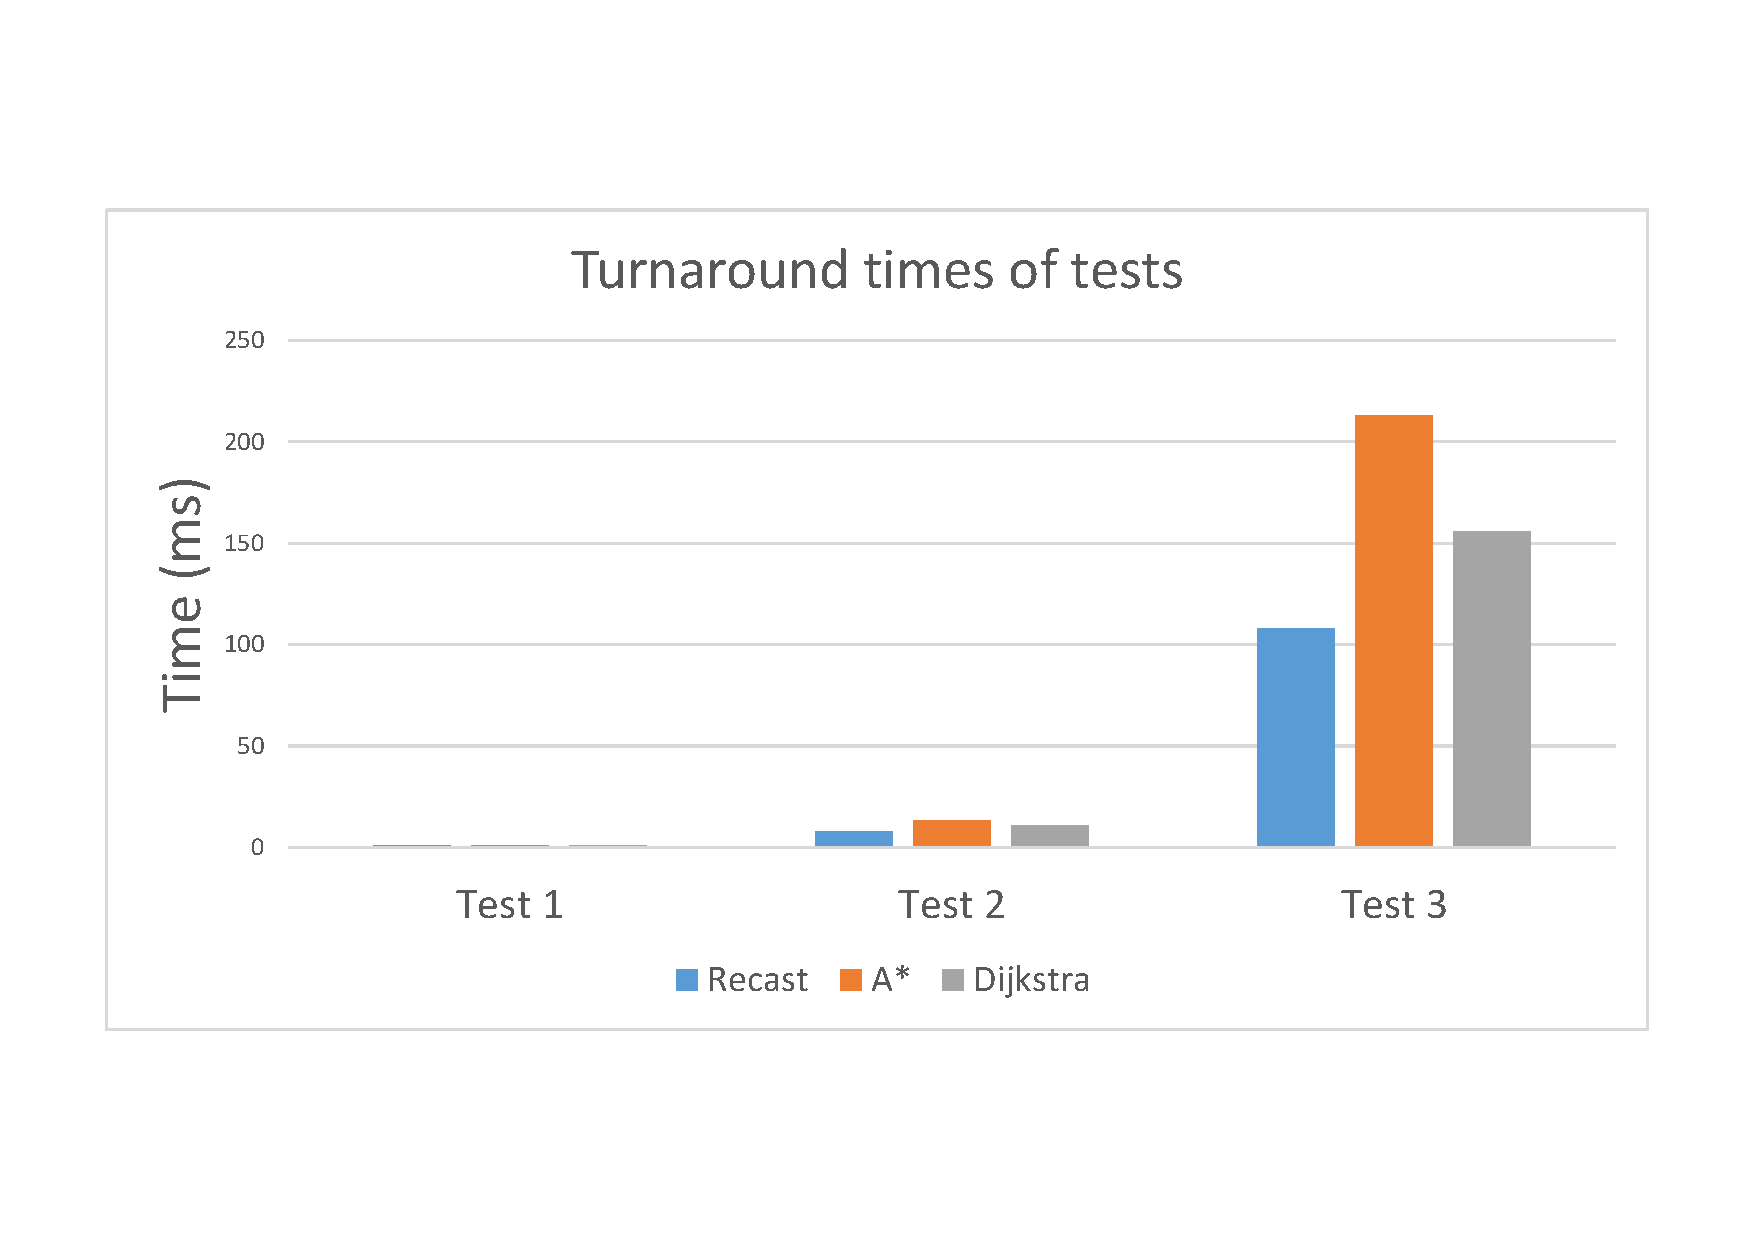
\includegraphics[trim=0 0 0 0, clip,width=0.8\textwidth,height=\textheight,keepaspectratio]{images/algoTurnaroundTimes.pdf}
\caption{Average times required by algorithms to return from computing tests.}
\label{fig:algoTurnaround}
\end{figure}

\begin{figure}[]
\center
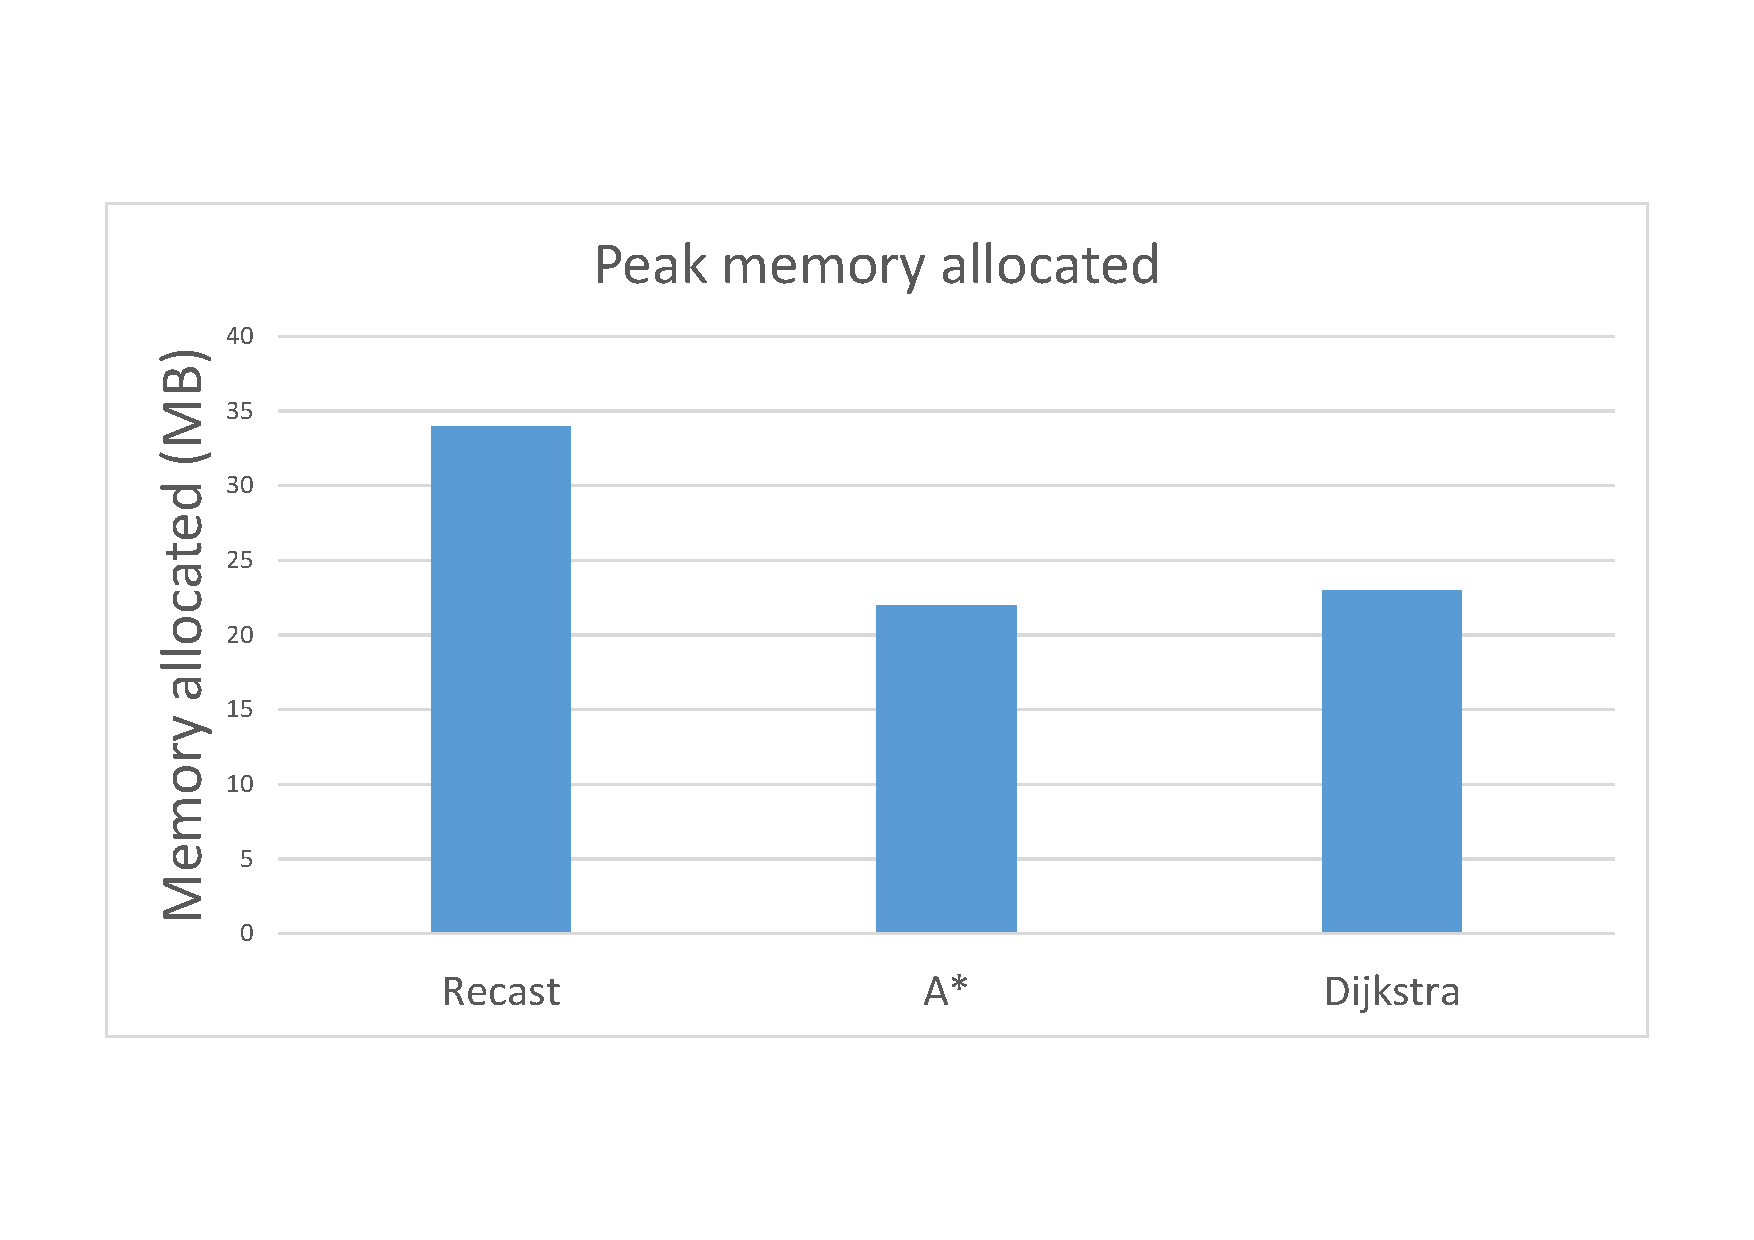
\includegraphics[trim=0 0 0 0, clip,width=0.8\textwidth,height=\textheight,keepaspectratio]{images/algoMemoryAlloc.pdf}
\caption{The maximum amount of memory specific algorithm (and libraries it loaded) required during its execution.}
\label{fig:algoMemAlloc}
\end{figure}

The results of our tests in figure[\ref{fig:algoTurnaround}] show that Recast is able to outperform both Dijkstra and A*, however it also comes with a significantly larger payload thanks to packing the whole Urho library with itself, as well as the memory required for pre-processing the graph. This therefore results in a 50\% larger memory requirement than the second highest competitor, Dijkstra. This can be seen in figure[\ref{fig:algoMemAlloc}]. While this might seem like a reasonable cost to pay for the performance benefit, for a mobile device (in which memory is a much more limited resource) it is too large. Therefore, we have decided to not go with Recast. Between A* and Dijkstra, the difference in memory allocated is negligible, and Dijkstra outperforms A* thanks to caching provided by the library. In our tests, A* also underperformed due to the large amount of walls in the floor plans, where it tried to utilize its predictive heuristic function to get closer to the target. From our testing we therefore decided to make use of the QuickGraph library, together with the provided Dijkstra observer. 

\end{document}
